\documentclass[border=4pt]{standalone}
\usepackage{mathptmx}
\usepackage{amsmath}
\usepackage{tikz}
\usetikzlibrary{positioning,arrows.meta,calc}
\begin{document}
\begin{minipage}{3.5in}
\centering
\resizebox{\linewidth}{!}{%
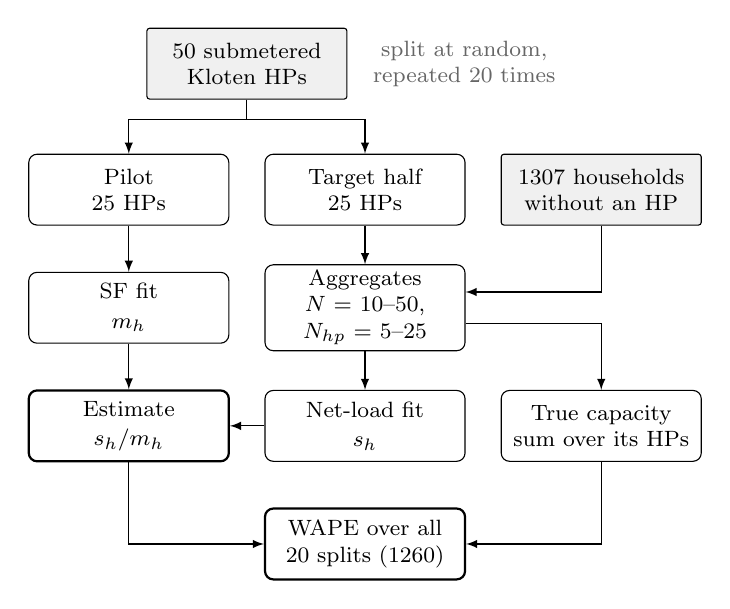
\begin{tikzpicture}[font=\footnotesize, >=latex,
  io/.style={draw, fill=black!6, rounded corners=1pt, align=center, text width=24mm, minimum height=9mm, inner sep=2pt},
  proc/.style={draw, rounded corners=3pt, align=center, text width=24mm, minimum height=9mm, inner sep=2pt},
  res/.style={draw, thick, rounded corners=3pt, align=center, text width=24mm, minimum height=9mm, inner sep=2pt},
  lab/.style={font=\footnotesize, text=black!60, align=center}]
% columns at x = 0, 30, 60 mm; rows top to bottom
\node[io]   (hps)   at (15mm, 0)      {50 submetered Kloten HPs};
\node[proc] (pilot) at (0, -16mm)     {Pilot\\25 HPs};
\node[proc] (half)  at (30mm, -16mm)  {Target half\\25 HPs};
\node[io]   (free)  at (60mm, -16mm)  {1307 households without an HP};
\node[proc] (sffit) at (0, -31mm)     {SF fit\\[1pt]$m_h$};
\node[proc] (agg)   at (30mm, -31mm)  {Aggregates\\$N$ = 10--50, $N_{hp}$ = 5--25};
\node[res]  (est)   at (0, -46mm)     {Estimate\\[1pt]$s_h / m_h$};
\node[proc] (net)   at (30mm, -46mm)  {Net-load fit\\[1pt]$s_h$};
\node[proc] (truth) at (60mm, -46mm)  {True capacity\\sum over its HPs};
\node[res]  (score) at (30mm, -61mm)  {WAPE over all\\20 splits (1260)};
% split
\node[lab, right=2mm of hps] {split at random,\\repeated 20 times};
\draw[->] (hps.south) -- ++(0,-2.5mm) -| (pilot.north);
\draw[->] (hps.south) -- ++(0,-2.5mm) -| (half.north);
% pilot branch
\draw[->] (pilot) -- (sffit);
\draw[->] (sffit) -- (est);
% target branch
\draw[->] (half) -- (agg);
\draw[->] (free.south) |- ([yshift=2mm]agg.east);
\draw[->] (agg) -- (net);
\draw[->] ([yshift=-2mm]agg.east) -| (truth.north);
\draw[->] (net) -- (est);
% scoring
\draw[->] (est.south) |- (score.west);
\draw[->] (truth.south) |- (score.east);
\end{tikzpicture}%
}
\par\smallskip
{\footnotesize Fig.~5.\ One split of the Kloten experiment. The pilot half gives $m_h$; aggregates drawn from the other half and the households without an HP give $s_h$ and their true capacity. No HP serves both the pilot and a target.}
\end{minipage}
\end{document}
